<latex>
\documentclass[12pt, a4paper]{article}
\usepackage[T2A]{fontenc}
\usepackage[utf8]{inputenc}
\usepackage[russian]{babel}
\usepackage{amsmath}
\usepackage{graphicx}
\setlength\parindent{0pt}
\usepackage[top=2cm,bottom=2cm,left=1.5cm,right=1.5cm]{geometry}
\onehalfspacing

\begin{document}

\subsubsection*{Гравитация. Сила тяжести.}
\[
F = G \,\frac{M\,m}{r^2},
\quad
g = G\,\frac{M_{\oplus}}{R_{\oplus}^2},
\quad
F = mg.
\]

\subsubsection*{Нормальная реакция опоры}
\[
\vec N \perp \text{поверхность}, 
\quad
N = mg,
\quad
N = m_{\rm сум} g,
\quad
P = N.
\]

\begin{center}
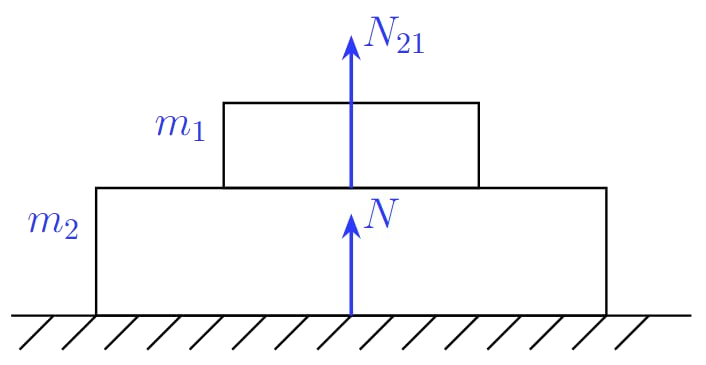
\includegraphics[width=0.33\linewidth]{7mgn.png}
\end{center}

\end{document}
</latex>